\begin{abstract}
	abstract
\end{abstract}

\section{Introduction}
\section{Data and Data preparation}
\section{Word Embeddings and Skip-Gram Model}
Natural Language Processing (NLP) tasks often benefit from representing words as vectors in a high-dimensional space.
 Word embeddings capture semantic and syntactic information about words, allowing models to reason about word relationships. While one-hot encoding is a simple approach, it fails to capture these important relationships.

 This section explores word embeddings and the Skip-Gram model,
 a popular method for learning word representations. The Skip-Gram model, proposed by Mikolov et al. \cite{word2vec}, predicts surrounding context words given a central word. This approach helps the model learn the semantic meaning of words based on their co-occurrence in text.
\subsection{Skip-Gram}
The Skip-Gram model, models the words representation by considering a center word $c$ and predicting $M$ words that are around $c$, the $M$ is refered as window size. The Figure \ref{fig:skipgram} illustrate a skipgram model with a window size of 2.

\begin{figure}[H]
	\begin{subfigure}{0.5\linewidth}
		\scalebox{0.8}{
			\tikzstyle{context} = [
				draw = black,
				fill = white,
				minimum size = 0.75cm
			]
			\tikzstyle{center} = [
				draw = black,
				fill = green!20,
				minimum size = 0.75cm
			]
		
			\begin{tikzpicture}[
				node distance = 0cm
			]
				\node  (pts1) at (0,0) {\ldots};
				\node [context, right=of pts1] (today) {today};
				\node [context, right=of today] (is) {is};
				\node [center, right=of is] (a) {a};
				\node [context, right=of a] (good) {good};
				\node [context, right=of good] (day) {day};
				\node [right=of day] (pts2) {\ldots};
				\path [->,>=latex](a.north) edge [bend left=50 ](good.north);
				\path [->,>=latex](a.north) edge [bend right=50 ](is.north);
				\path [->,>=latex](a.north) edge [bend right=50 ](today.north);
				\path [->,>=latex](a.north) edge [bend left =50](day.north);


				\node  (pts1) at (0,-2) {\ldots};
				\node [context, right=of pts1] (today) {today};
				\node [context, right=of today] (is) {is};
				\node [context, right=of is] (a) {a};
				\node [center, right=of a] (good) {good};
				\node [context, right=of good] (day) {day};
				\node [right=of day] (pts2) {\ldots};
				\path [->,>=latex](good.north) edge [bend right=50 ](a.north);
				\path [->,>=latex](good.north) edge [bend right=50 ](is.north);
				% \path [->,>=latex](good.north) edge [bend right=50 ](today.north);
				\path [->,>=latex](good.north) edge [bend left =50](day.north);
			\end{tikzpicture}}
	\caption{Skip-Gram Illustraion}
	\end{subfigure}\begin{subfigure}{0.5\linewidth}
		\scalebox{0.8}{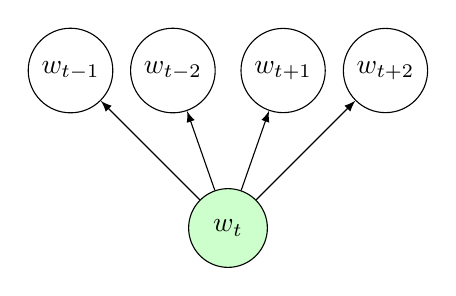
\begin{tikzpicture}[
			node distance = 0.75cm,
			every node/.style = {
				draw = black,
				minimum size = 0.75cm,
				circle
			},
			every edge/.style = {
				-Stealth
			}
		]
			
			\node[minimum size=1cm, fill=green!20] (center)  at (0,0) {$w_t$};
			
			\node(w1)  at (-2,2) {$w_{t-1}$};
			\node(w2) at (-0.7,2){$w_{t-2}$};
			\node(w3) at (0.7, 2) {$w_{t+1}$};
			\node(w4) at (2,2) {$w_{t+2}$};
			
			\draw[->, >=latex] (center) -- (w1);
			\draw[->, >=latex] (center) -- (w2);
			\draw[->, >=latex] (center) -- (w3);
			\draw[->, >=latex] (center) -- (w4);
		\end{tikzpicture}
}		\caption{Skip-Gram Model}
	\end{subfigure}
	\caption{The skip-gram model}
	\label{fig:skipgram}
\end{figure}

In other words, we compute $p(w_{t-2}, w_{t-1}, w_{t+1}, w_{t+2} | w_t)$. The following assumptions simplify the model:
\begin{itemize}
    \item Each window is an identically and independently distributed sample.
    \item Within each window, each context word is conditionally independent given the center word.
    \item Each context word can be predicted from the center word in the same way, irrespective of its position.
\end{itemize}
Considering the sequence $w_{1:T}$ and a window size $M$, we can derive the negative likelihood of our model written as follows, with the two first assumptions:
\begin{align}
J(\mbf{\theta}) &= -\log\prod_{t=1}^{T}P_{\mathbf{\theta}}(w_{t-M:t-1},w_{t+1:t+M}|w_t)\\
&=-\sum_{t=1}^{T}\sum_{\substack{-M\leq j \leq M,\\ j\neq 0}}\log P_{\mathbf{\theta}}(w_{t+j}|w_t)
\end{align}

To obtain $P_{\mathbf{\theta}}(w_{t+j}|w_t)$ we consider the third assumption. We also denote the vector represntation of a context word $w$ $\mbf{u}_w$, and $\mbf{v}_w$ if $w$ is centre word. Then for a centre word $c$ and context word $o$, we have:
\begin{equation}
	P_{\mathbf{\theta}}(w_{t+j}=o|w_t=c) = P(o|c) = \frac{e^{\mbf{u}_o^\top\mbf{v}_c}}{\sum_{w\in \mathcal{V}}e^{\mbf{u}_{w}^\top\mbf{v}_c}}
\end{equation}
where $\mathcal{V}$ is the set of vocabulary. By denoting $\mbf{f_\theta}(\cdot)$ our, model, then for a centre word $c$ we have
\begin{equation}
	\mbf{f_\theta}(w_t=c)=\frac{1}{\sum_{w\in \mathcal{V}}e^{\mbf{u}_{w}^\top\mbf{v}_c}}\begin{bmatrix}
		e^{\mbf{u}_o^\top\mbf{v}_c}\\
		e^{\mbf{u}_o^\top\mbf{v}_c}\\
		\vdots\\
		e^{\mbf{u}_o^\top\mbf{v}_c}\\
	\end{bmatrix}
	= \softmax\left(\mbf{Uv}_c\right)
\end{equation}
In that model, the parameters are two $D \times |\mathcal{V}|$ matrices, $\mbf{U}$ and $\mbf{V}$, where each column of $\mbf{U}$ represents the vector embedding of a word in the vocabulary as a context word, and each column of $\mbf{V}$ represents the vector embedding of a word in the vocabulary as a center word.

Then, to find the optimal parameters, we can use Gradiend descent or its variant to find the optimal parameters by minimizing the negative log likelihood $J(\mbf{\theta})$.

One of the major issue of with this approach is the computational complexity induced by the softmax, when we deal with a big dataset. A solution to this is proposed in \cite{sgns} that we will present in the next section.
\subsection{Improved Word2vec with subsampling and negative sampling}
Some words in the corpus have a high frequency, but irrevelents than some rare words. To address this imbalance and focus on more informative words,
we can discard some frequent words using a heuristic probability:
\begin{equation}
	p(w_i) = 1-\sqrt{\frac{t}{f(w_i)}}
\end{equation}
Where $f(w_i)$ if the frequency of the word $w_i$, and $t$ a choosen threshold suggested to be $10^{-5}$. By doing this, we reduce the size of our vocabulary while keeping more informative words.



On the other hand, from the Noise Contrastive Estimation says that a good model should be able to differntiate data from noise by the mean of a logistic regression \cite{sgns}. Based on that, for each pair $(c, o)$ (positive) we sample $K$  pairs $(c, w_i)$ (negatives) then our model should predict if a given pair is  a valid pair i.e, a valid centre context words or not. Thus, for a single pair we have the following negative log likelihood:
\begin{equation}
J_{c,o}(\mbf{\theta}) = -\log\sigma(\mbf{u}_o^\top\mbf{v}_c) - \sum_{i=1}^{k}\log\sigma(\mbf{u}_{w_i}^\top\mbf{v}_c)
\end{equation}
This approcah reduce the computaion of a big softmax into sevaral sigmoid.

\subsection{Words embedding evaluation}
This section discusses how to evaluate word embeddings and their usage in text classification.
Cosine similarity is a common metric used to measure the similarity between two word embeddings, denoted by $\mbf{u}$ and $\mbf{v}$. It is defined as:

\begin{equation}
	\cos(\mbf{u}, \mbf{v}) =\frac{\mbf{u}^\top \mbf{v}}{\|\mbf{u}\|\|\mbf{v}\|}\in [-1,1]
\end{equation}
Words with similar meanings will have a cosine similarity close to 1, while dissimilar words will have a value closer to -1. Additionally, the distance between two embeddings can be calculated using:
\begin{equation}
	\mathrm{d}(\mbf{u}, \mbf{v}) =1 -\cos(\mbf{u}, \mbf{v})\in [0,2]
\end{equation}
However, evaluating the overall quality of word embeddings is a complex task. Here are two common approaches:
\begin{itemize}
	\item \textbf{Visualization:} Techniques like PCA, t-SNE, UMAP can be used to project word embeddings into a lower-dimensional space for visual inspection. By looking at known similar words and how they cluster together, we can gain insights into the quality of the embeddings.
	\item \textbf{Intrinsic Evaluation:} This involves evaluating the model's ability to capture semantic relationships between words. We can compare the cosine similarity of known synonym or analogy pairs with the model's predictions.
\end{itemize}



\subsection{Text Classification}
One powerful application of word embeddings is text classification. We can leverage the embedding vectors to represent the meaning of an entire sentence.
\begin{equation}
	\mbf{w}_{\mathrm{sentence}} = \frac{1}{T}\sum_{T}^{t=1}\mbf{w}_t
\end{equation}
where $\mbf{w}_t$ is the embedding of the t\textsuperscript{th} word and T is the total number of words.
This sentence embedding is then fed into a text classifier to predict its category. 
\section{Results and Discussion}
\section{Conclusion}

\begin{thebibliography}{1}

	\bibitem{kamper2022nlp817}
	Herman Kamper. \emph{NLP817}. \href{https://www.kamperh.com/nlp817/}{https://www.kamperh.com/nlp817/}, 2022--2024.
	
	\bibitem{word2vec} Mikolov, T., Chen, K., Corrado, G. and Dean, J., 2013. Efficient estimation of word representations in vector space. \textit{arXiv preprint arXiv:1301.3781}.

	\bibitem{sgns} Mikolov, T., Sutskever, I., Chen, K., Corrado, G.S. and Dean, J., 2013. Distributed representations of words and phrases and their compositionality. \textit{Advances in neural information processing systems, 26}.
	
	\end{thebibliography}